\setcounter{ExampleCounter}{1}
A logical argument builds a conclusion from a set of \textit{premises}.\marginnote{Premise: the basis of an argument or proof}  Our job in this section will be to sift through various arguments and find which are valid and which are invalid.\\

There are two basic types of arguments: inductive and deductive.  We'll focus in this section on deductive arguments, but here we'll give a few examples of inductive arguments for the sake of interest.  The difference between an inductive argument and a deductive argument is that an inductive argument builds from specific examples to draw a general principle, and a deductive argument is the reverse, using a general principle to imply specific examples.\\

\begin{proc}{Argument Types}
An \textbf{inductive argument} uses a collection of specific examples as its premises and proposes a general principle as its conclusion.
\begin{center}
{\Large
\begin{tabular}{r c l}
Specific & $\longrightarrow$ & General\\
& & 
\end{tabular}}
\end{center}

A \textbf{deductive argument} uses one or more general principles as its premises and proposes a specific situation as its conclusion.
\begin{center}
{\Large
\begin{tabular}{r c l}
General & $\longrightarrow$ & Specific
\end{tabular}}
\end{center}
\end{proc}

\begin{example}[https://www.youtube.com/watch?v=F7w7wOvpntA]{Inductive Argument}
The following is an example of an inductive argument:\\
``When I went to the store last week I forgot my wallet, and when I went today I forgot my wallet.  I always forget my wallet when I go to the store.''\\

\textbf{Premises:}\marginnote{Specific examples}\\
I forgot my wallet last week.\\
I forgot my wallet today.\\

\textbf{Conclusion:}\marginnote{General principle}\\
I always forget my wallet.\\

This is a fairly weak argument, since it is based on only two instances.
\end{example}

An example of a stronger inductive argument is one like the following:
\begin{center}
Every day for the past year, a plane has flown over my house at 2 pm.\\
A plane will fly over my house every day at 2 pm.
\end{center}
This is a stronger argument because it has a larger set of specific examples to support the conclusion.\\

Inductive arguments can never prove the conclusion true, but it can provide evidence to suggest that it may be true.  This evidence tends to be stronger if there are more examples.

Every medical study is an example of an inductive argument.  For instance, to test a new blood pressure medication, a pharmaceutical company might design a trial with 100 patients with high blood pressure.  If they give half of them the new medication, and that half experiences a dramatic improvement in blood pressure, they can conclude that the medication accomplishes their goal.  While that doesn't technically \textit{prove} that claim by a logical standard, it provides strong enough evidence that the company can confidently market the new drug.

Unlike inductive arguments, deductive arguments can be definitively analyzed for validity.
\vfill
\pagebreak

\begin{example}[https://www.youtube.com/watch?v=TIVWCVyZrVw]{Deductive Argument}
\newcounter{dedarg}
\setcounter{dedarg}{\theExampleCounter}
The following is an example of a deductive argument:\\
``All cats are mammals.  Since a tiger is a cat, a tiger is a mammal.''\\

\textbf{Premises:}\marginnote{General principles}\\
All cats are mammals.\\
A tiger is a cat.\\

\textbf{Conclusion:}\marginnote{Specific example}\\
A tiger is a mammal.
\end{example}

A valid argument\marginnote{For the rest of this section, the word \textit{argument} will refer to \textit{deductive argument}.} is one that has a solid chain of implication leading from the premises to the conclusion.\\

\begin{proc}{Valid Deductive Argument}
A deductive argument is considered \textbf{valid} if the conclusion follows logically from the premises.  In other words, an argument is valid if the conclusion is true whenever the premises are true.\\

We will evaluate the validity of deductive arguments in two ways:
\begin{enumerate}
\item Using diagrams
\item Building truth tables
\end{enumerate}
\end{proc}

Notice that when we say that an argument is \textbf{valid}, we don't focus on whether or not the premises are true; we just want to prove that IF they are true, the conclusion must logically follow.  We can also talk about \textbf{true} arguments, which are valid arguments with premises that are provably true.

We need to start with a valid argument, though, and then we can start to investigate whether the premises are true or not.

\subsection{Evaluating Arguments With Diagrams}
\begin{example}[https://www.youtube.com/watch?v=j49KYvFiPUQ]{Evaluating an Argument with a Diagram}
Consider the argument from example \thededarg:\\
``All cats are mammals.  Since a tiger is a cat, a tiger is a mammal.''\\

The first premise, that all cats are mammals, is a quantified statement using the universal quantifier.  We\marginnote{This is called an \textit{Euler diagram}, named for Leonhard Euler.} drew a diagram like the one below to illustrate statements like this.  Saying that all cats are mammals is the same as saying that the set of cats is a subset of the set of mammals.
\begin{center}
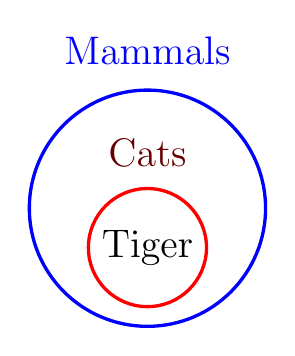
\begin{tikzpicture}
  %\draw [very thick,color=orange!30!black, fill=orange!20] (-3cm,-2cm) rectangle (3cm,2.6cm);

  \draw [very thick,color=blue, fill=white] (0,0) circle (1.5cm);
  \draw [yshift=2cm,xshift=0cm] node {\color{blue}\Large Mammals};
  
  \draw [very thick,color=red, fill=white] (0,-0.5) circle (0.75cm);
  \draw [yshift=0.7cm,xshift=0cm] node {\color{red!40!black}\Large Cats};
  
  \draw [yshift=-0.5cm,xshift=0cm] node {\color{black}\Large Tiger};
\end{tikzpicture}
\end{center}
The second premise, that a tiger is a cat, places the tiger within the circle that represents cats.  Clearly, the tiger must also lie in the circle that represents mammals, so this argument is valid.
\end{example}

Typically, arguments with premises that involve the universal quantifier like this one are handled naturally with diagrams.

\begin{example}[https://www.youtube.com/watch?v=HkTBaUzay4g]{Evaluating an Argument with a Diagram}
Argument:\\
``All firefighters know CPR.  Jill knows CPR.  Therefore, Jill is a firefighter.''\\

\textbf{Premises:}\\
All firefighters know CPR.\\
Jill knows CPR.\\

\textbf{Conclusion:}\\
Jill is a firefighter.\\

Based on the first premise, the set of firefighters must lie within the set of those who know CPR.  Based on the second premise, Jill is somewhere in the circle of those who know CPR, but it isn't clear whether she is inside the firefighter set.

\begin{center}
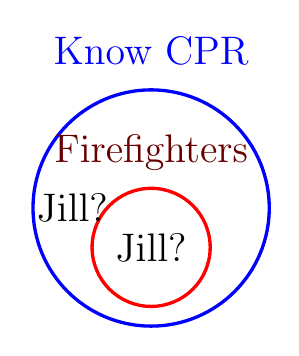
\begin{tikzpicture}
  %\draw [very thick,color=orange!30!black, fill=orange!20] (-3cm,-2cm) rectangle (3cm,2.6cm);

  \draw [very thick,color=blue, fill=white] (0,0) circle (1.5cm);
  \draw [yshift=2cm,xshift=0cm] node {\color{blue}\Large Know CPR};
  
  \draw [very thick,color=red, fill=white] (0,-0.5) circle (0.75cm);
  \draw [yshift=0.7cm,xshift=0cm] node {\color{red!40!black}\Large Firefighters};
  
  \draw [yshift=-0.5cm,xshift=0cm] node {\color{black}\Large Jill?};
  \draw [yshift=0cm,xshift=-1cm] node {\color{black}\Large Jill?};
\end{tikzpicture}
\end{center}

Therefore, this argument is not valid, because just being in the set of those who know CPR is not enough to guarantee being in the set of firefighters.
\end{example}

\begin{try}
Is the following argument valid or not?
\begin{center}
``No cows are purple.  Fido is not a cow, so Fido is purple.''
\end{center}
\end{try}

\subsection{Evaluating Arguments With Truth Tables}
As we've seen, arguments that involve claims about quantified statements are often easy to visualize with diagrams, as in the examples above.

If, on the other hand, an argument involves conditional statements, it is more natural to analyze the argument with a truth table.  Remember, an argument is valid if the conclusion is true every time the premises are true.  We'll build a truth table to see if the premises lead to the conclusion every time they're true.

\begin{proc}{Evaluating Arguments With Truth Tables}
An argument is valid if the premises imply the conclusion.  Thus, to analyze an argument, we can construct a truth table for the statement 
\[[(\textrm{premise 1}) \wedge (\textrm{premise 2}) \wedge \ldots (\textrm{premise } n)] \to \textrm{ conclusion}.\]

If this column is all true, that means that the premises DO imply the conclusion for every possibility, so the argument is valid.  If there is at least one false value in this column, the argument is invalid.
\end{proc}

\begin{formula}{Fallacies}
An invalid argument is called a \textbf{fallacy}.
\end{formula}

\begin{example}[https://www.youtube.com/watch?v=IWk35nPpq3g]{Evaluating an Argument with a Truth Table}
Consider the following argument:\\
``If you take a lot of math classes, you will lose sleep.  You are taking a lot of math classes.  Therefore, you will lose sleep.''

\sol
This is a simple example, and it should be obvious that this is a valid argument, but we'll use this to illustrate the process of testing an argument by building a truth table.

First, define the premises and conclusion:\\

\textbf{Premises:}\marginnote{In words}\\
If you take a lot of math classes, you will lose sleep.\\
You are taking a lot of math classes.\\

\textbf{Conclusion:}\\
You will lose sleep.\\

Let's define the simple statements that appear in the premises and conclusion:\\
$p$: ``You take a lot of math classes.''\\
$q$: ``You lose sleep.''\\

We can now write the argument more concisely using these letters to represent the statements:\\

\textbf{Premises:}\marginnote{Symbolically}\\
$p \to q$\\
$p$\\

\textbf{Conclusion:}\\
$q$\\

The full argument is $[(p \to q) \wedge p] \to q$.  We will now build a truth table for this argument.
\begin{center}
\begin{tabular}{|c c c c c|}
\hline
$p$ & $q$ & $p \to q$ & $(p \to q) \wedge p$ & $[(p \to q) \wedge p] \to q$\\
\hline
& & & & \\
T & T & T & T & T\\
T & F & F & F & T\\
F & T & T & F & T\\
F & F & T & F & T\\
\hline
\end{tabular}
\end{center}
Since the last column is all true values, we've proven that this argument is valid.
\end{example}

\begin{try}
Determine if the following argument is valid.\\

\textbf{Premises:}\\
If I have a shovel I can dig a hole.\\
I dug a hole.\\

\textbf{Conclusion:}\\
Therefore, I had a shovel.
\end{try}
\vfill
\pagebreak

\begin{example}[https://www.youtube.com/watch?v=pCnvn2-nENk]{Evaluating an Argument with a Truth Table}
Is the following argument valid, or is it a fallacy?\\

``If the defendant's DNA is found at the crime scene, then we can have him stand trial.  He is standing trial.  Consequently, we have found evidence of his DNA at the crime scene.''

\sol
\textbf{Premises:}\\
\begin{tabular}{l l}
$p \to q$: & If his DNA is found at the crime scene, we can have him stand trial.\\
$q$: & He is standing trial.\\
& \\
\end{tabular}

\textbf{Conclusion:}\\
\begin{tabular}{l l}
$q$: & We found evidence of his DNA at the crime scene.
\end{tabular}

The structure of the argument is \[[(p \to q) \wedge q] \to p\]
which can be analyzed with the following truth table.
\begin{center}
\begin{tabular}{|c c c c c|}
\hline
$p$ & $q$ & $p \to q$ & $(p \to q) \wedge q$ & $[(p \to q) \wedge q] \to p$\\
\hline
& & & & \\
T & T & T & T & T\\
T & F & F & F & T\\
F & T & T & T & F\\
F & F & T & F & T\\
\hline
\end{tabular}
\end{center}

Since a false value appears in the last column, this argument is a fallacy.
\end{example}

Notice the fallacy in the last example.  When we make a statement like ``If the defendant's DNA is found at the crime scene, we can have him stand trial,'' we are not excluding the possibility that something else could lead to him standing trial.  Thus, just knowing that he's standing trial is not enough to conclude that his DNA was found.  In fact, looking at the truth table, we can see that the one case where the argument breaks down is the case where $p$ is false, and $q$ is true, meaning the case where his DNA was not found at the crime scene and yet he is standing trial.

\subsection{Common Valid and Invalid Arguments}
There are several common valid arguments and common fallacies, and we'd like to be able to recognize them.  If we can strip an argument down to its basic form and match it to one of these common forms, we won't have to build a truth table every time.  This way, we'll be able to analyze and build arguments much more efficiently.

Notice that we've already seen an example of a valid argument and a fallacy.  These two are common forms called, respectively, direct reasoning and the fallacy of the converse.

\begin{formula}{Direct Reasoning and the Fallacy of the Converse}
A valid argument using \textbf{direct reasoning}\marginnote{This argument form is sometimes called \textit{modus ponens}, which is Latin for ``method of affirming.''} follows the pattern
\begin{center}
\begin{tabular}{l l}
$p \to q$ & Premise\\
$p$ & Premise\\
\hline
& \\
$\therefore\marginnote{The symbol $\therefore$ means ``therefore''} q$ & Conclusion
\end{tabular}
\end{center}

The \textbf{fallacy of the converse} follows the pattern
\begin{center}
\begin{tabular}{l}
$p \to q$\\
$q$\\
\hline
$\therefore p$
\end{tabular}
\end{center}
\end{formula}

The fallacy of the converse tries to turn a conditional statement around and make the implication imply the condition.

We'll look at other pairs like this, valid arguments and the fallacies that look similar to them.
\vfill
\pagebreak

\begin{example}[https://www.youtube.com/watch?v=UTm75PK8uSs]{Valid and Invalid Arguments}
Is the following argument valid, or is it a fallacy?\\

``If my computer crashes, I'll lose all my photos.  I haven't lost all my photos.  Therefore, my computer hasn't crashed.''

\sol
\textbf{Premises:}\\
\begin{tabular}{l l}
$p \to q$: & If my computer crashes, I'll lose all my photos.\\
$\sim q$: & I haven't lost all my photos.\\
& \\
\end{tabular}

\textbf{Conclusion:}\\
\begin{tabular}{l l}
$\sim p$: & My computer hasn't crashed.
\end{tabular}

The structure of the argument is \[[(p \to q) \wedge \sim q] \to \sim p\]
which can be analyzed with the following truth table.
\begin{center}
\begin{tabular}{|c c c c c c c|}
\hline
$p$ & $q$ & $\sim p$ & $\sim q$ & $p \to q$ & $(p \to q) \wedge \sim q$ & $[(p \to q) \wedge \sim q] \to \sim p$\\
\hline
& & & & & & \\
T & T & F & F & T & F & T\\
T & F & F & T & F & F & T\\
F & T & T & F & T & F & T\\
F & F & T & T & T & T & T\\
\hline
\end{tabular}
\end{center}

Since the last column is all T's, the argument is valid.  This is an example of \textbf{contrapositive reasoning}.
\end{example}

\begin{example}[https://www.youtube.com/watch?v=QS_cuap6hy0]{Valid and Invalid Arguments}
Is the following argument valid, or is it a fallacy?\\

``If I am at the beach, then I get sunburned.  I'm not at the beach, so I won't get sunburned.''

\sol
\textbf{Premises:}\\
\begin{tabular}{l l}
$p \to q$: & If I'm at the beach, I get sunburned\\
$\sim p$: & I'm not at the beach.\\
& \\
\end{tabular}

\textbf{Conclusion:}\\
\begin{tabular}{l l}
$\sim q$: & I won't get sunburned.
\end{tabular}

The structure of the argument is \[[(p \to q) \wedge \sim p] \to \sim q\]
which can be analyzed with the following truth table.
\begin{center}
\begin{tabular}{|c c c c c c c|}
\hline
$p$ & $q$ & $\sim p$ & $\sim q$ & $p \to q$ & $(p \to q) \wedge \sim p$ & $[(p \to q) \wedge \sim p] \to \sim q$\\
\hline
& & & & & & \\
T & T & F & F & T & F & T\\
T & F & F & T & F & F & T\\
F & T & T & F & T & T & F\\
F & F & T & T & T & T & T\\
\hline
\end{tabular}
\end{center}

Since the last column contains an F, this argument is a fallacy.  This is an example of the \textbf{fallacy of the inverse}.
\end{example}

\begin{try}
What form does the following argument match?

``If you jump off that cliff, you'll break your leg.''\\  ``I won't jump off the cliff, so I won't break my leg.''
\end{try}

\begin{formula}{Contrapositive Reasoning and the Fallacy of the Inverse}
A valid argument using \textbf{contrapositive reasoning}\footnote{This argument form is much less intuitive than direct reasoning, but very powerful.}\marginnote{This argument form is sometimes called \textit{modus tollens}, which is Latin for ``method of denying.''} follows the pattern
\begin{center}
\begin{tabular}{l}
$p \to q$\\
$\sim q$\\
\hline
$\therefore\ \sim p$
\end{tabular}
\end{center}

The \textbf{fallacy of the inverse} follows the pattern
\begin{center}
\begin{tabular}{l}
$p \to q$\\
$\sim p$\\
\hline
$\therefore\ \sim q$
\end{tabular}
\end{center}
\end{formula}

The next pair of arguments don't involve conditional statements; instead, they involve an OR statement, sometimes called a \textit{disjunction}.

\begin{example}[https://www.youtube.com/watch?v=6DtnGoYXgjY]{Valid and Invalid Arguments}
Is the following argument valid, or is it a fallacy?\\

``I'm either cold or hot.  I'm not cold, so I am hot.''

\sol
\textbf{Premises:}\\
\begin{tabular}{l l}
$p \vee q$: & I'm either cold or hot.\\
$\sim p$: & I'm not cold.\\
& \\
\end{tabular}

\textbf{Conclusion:}\\
\begin{tabular}{l l}
$q$: & I am hot.
\end{tabular}

The structure of the argument is \[[(p \vee q) \wedge \sim p] \to q\]
which can be analyzed with the following truth table.
\begin{center}
\begin{tabular}{|c c c c c c|}
\hline
$p$ & $q$ & $\sim p$ & $p \vee q$ & $(p \vee q) \wedge \sim p$ & $[(p \vee q) \wedge \sim p] \to q$\\
\hline
& & & & & \\
T & T & F & T & F & T\\
T & F & F & T & F & T\\
F & T & T & T & T & T\\
F & F & T & F & F & T\\
\hline
\end{tabular}
\end{center}

This is a valid argument, called \textbf{disjunctive reasoning}.  Essentially, this argument says that there are only two alternatives, $p$ and $q$.  If one of them is not true, the other must be.
\end{example}

\begin{example}[https://www.youtube.com/watch?v=uYJbdR7-uQU]{Valid and Invalid Arguments}
Is the following argument valid, or is it a fallacy?\\

``A musician can play the guitar or the piano.  She can play the guitar, so she can't play the piano.''

\sol
\textbf{Premises:}\\
\begin{tabular}{l l}
$p \vee q$: & She can play the guitar or she can play the piano.\\
$p$: & She can play the guitar.\\
& \\
\end{tabular}

\textbf{Conclusion:}\\
\begin{tabular}{l l}
$\sim q$: & She can't play the piano.
\end{tabular}

The structure of the argument is \[[(p \vee q) \wedge p] \to \sim q.\]
\vfill
\pagebreak

The following truth table analyzes this argument.
\begin{center}
\begin{tabular}{|c c c c c c|}
\hline
$p$ & $q$ & $\sim q$ & $p \vee q$ & $(p \vee q) \wedge p$ & $[(p \vee q) \wedge p] \to \sim q$\\
\hline
& & & & & \\
T & T & F & T & T & F\\
T & F & T & T & T & T\\
F & T & F & T & F & T\\
F & F & T & F & F & T\\
\hline
\end{tabular}
\end{center}

This is a fallacy, called \textbf{misuse of disjunctive reasoning}. 
\end{example}

\begin{formula}{Disjunctive Reasoning and Its Misuse}
A valid argument using \textbf{disjunctive reasoning}\marginnote{Either $p$ or $q$ is true.  If we know that one isn't true, the other must be.} follows the pattern
\begin{center}
\begin{tabular}{l c l}
\begin{tabular}{l}
$p \vee q$\\
$\sim p$\\
\hline
$\therefore q$
\end{tabular} & OR &
\begin{tabular}{l}
$p \vee q$\\
$\sim q$\\
\hline
$\therefore p$
\end{tabular}
\end{tabular}
\end{center}

A fallacy called the \textbf{misuse of disjunctive reasoning}\marginnote{This ignores the fact that the OR is inclusive; $p$ can be true or $q$ can be true or both can be true.} follows the pattern
\begin{center}
\begin{tabular}{l c l}
\begin{tabular}{l}
$p \vee q$\\
$p$\\
\hline
$\therefore\ \sim q$
\end{tabular} & OR &
\begin{tabular}{l}
$p \vee q$\\
$q$\\
\hline
$\therefore\ \sim p$
\end{tabular}
\end{tabular}
\end{center}
\end{formula}

\begin{example}[https://www.youtube.com/watch?v=0M57bPxQOKg]{Valid and Invalid Arguments}
Is the following argument valid, or is it a fallacy?\\

``If you wear an enormous cowboy hat, people will stare.  If people stare at you, you get embarrassed.  Therefore, if you wear an enormous cowboy hat, you will be embarrassed.''

\sol
\textbf{Premises:}\\
\begin{tabular}{l l}
$p \to q$: & If you wear an enormous cowboy hat, people will stare.\\
$q \to r$: & If people stare at you, you get embarrassed.\\
& \\
\end{tabular}

\textbf{Conclusion:}\\
\begin{tabular}{l l}
$p \to r$: & If you wear an enormous cowboy hat, you will be embarrassed.
\end{tabular}

The structure of the argument is \[[(p \to q) \wedge (q \to r)] \to (p \to r)\]
which can be analyzed with the following truth table.
\begin{center}
{\small
\begin{tabular}{|c c c c c c c c|}
\hline
$p$ & $q$ & $r$ & $p \to q$ & $q \to r$ & $p \to r$ & $(p \to q) \wedge (q \to r)$ & $[(p \to q) \wedge (q \to r)] \to (p \to r)$\\
\hline
& & & & & & & \\
T & T & T & T & T & T & T & T\\
T & F & T & F & T & T & F & T\\
F & T & T & T & T & T & T & T\\
F & F & T & T & T & T & T & T\\
T & T & F & T & F & F & F & T\\
T & F & F & F & T & F & F & T\\
F & T & F & T & F & T & F & T\\
F & F & F & T & T & T & T & T\\
\hline
\end{tabular}}
\end{center}

This is a valid argument, called \textbf{transitive reasoning}.  Transitive reasoning means stringing conditional statements together, where the conclusion of one statement forms the condition of the next.  As long as we can form a chain like these, we can string many conditional statements together and have a valid conclusion that leads from the beginning to the end.
\end{example}
\vfill
\pagebreak

\begin{example}[https://www.youtube.com/watch?v=ocJ0y5qimTY]{Valid and Invalid Arguments}
Is the following argument valid, or is it a fallacy?\\

``If you watch \textit{Old Yeller}, you will cry.  If you cry, your shirt will be stained.  Your shirt is stained, so you must have watched \textit{Old Yeller}.''

\sol
\textbf{Premises:}\\
\begin{tabular}{l l}
$p \to q$: & If you watch \textit{Old Yeller}, you will cry.\\
$q \to r$: & If you cry, your shirt will be stained.\\
& \\
\end{tabular}

\textbf{Conclusion:}\\
\begin{tabular}{l l}
$r \to p$: & Your shirt is stained, so you must have watched \textit{Old Yeller}.
\end{tabular}

The structure of the argument is \[[(p \to q) \wedge (q \to r)] \to (r \to p)\]
which can be analyzed with the following truth table.
\begin{center}
{\small
\begin{tabular}{|c c c c c c c c|}
\hline
$p$ & $q$ & $r$ & $p \to q$ & $q \to r$ & $r \to p$ & $(p \to q) \wedge (q \to r)$ & $[(p \to q) \wedge (q \to r)] \to (r \to p)$\\
\hline
& & & & & & & \\
T & T & T & T & T & T & T & T\\
T & F & T & F & T & T & F & T\\
F & T & T & T & T & F & T & F\\
F & F & T & T & T & F & T & F\\
T & T & F & T & F & T & F & T\\
T & F & F & F & T & T & F & T\\
F & T & F & T & F & T & F & T\\
F & F & F & T & T & T & T & T\\
\hline
\end{tabular}}
\end{center}

This is a fallacy, called \textbf{misuse of transitive reasoning}.  The correct conclusion to this argument is $p \to r$, so concluding that $r \to p$ means thinking that the conditional statement and its converse are equivalent, which we have shown before that they are not.
\end{example}

\begin{formula}{Transitive Reasoning and Its Misuse}
A valid argument using \textbf{transitive reasoning} follows the pattern
\begin{center}
\begin{tabular}{l c l}
\begin{tabular}{l}
$p \to q$\\
$q \to r$\\
\hline
$\therefore p \to r$
\end{tabular} & OR &
\begin{tabular}{l}
$p \to q$\marginnote{Note: the two forms shown are equivalent, because a conditional statement $p \to r$ and its contrapositive $\sim r \to\ \sim p$ are equivalent.}\\
$q \to r$\\
\hline
$\therefore\ \sim r \to\ \sim p$
\end{tabular}
\end{tabular}
\end{center}

A fallacy called the \textbf{misuse of transitive reasoning} tries to build a transitive chain, but fails.  One possibility form for this fallacy is the following.
\begin{center}
\begin{tabular}{l c l}
\begin{tabular}{l}
$p \to q$\\
$q \to r$\\
\hline
$\therefore r \to p$
\end{tabular} & OR &
\begin{tabular}{l}
$p \to q$\\
$q \to r$\\
\hline
$\therefore\ \sim p \to\ \sim r$
\end{tabular}
\end{tabular}
\end{center}

The difference between transitive reasoning and its misuse can often be subtle in words, but it is clearer when we break down the argument.  Notice that there are multiple ways to misuse transitive reasoning; only the chain of implication shown above is valid.  Other arguments that look like transitive reasoning can be analyzed the same way that we analyzed the previous example.
\end{formula}

\begin{try}
Is the following argument valid?\\

\textbf{Premises:}\\
If I go to the party, I'll be really tired tomorrow.\\
If I go to the party, I'll get to see friends.\\

\textbf{Conclusion:} If I don't see friends, I won't be tired tomorrow.
\end{try}

\begin{example}[https://www.youtube.com/watch?v=IbjD73wapPs]{Valid and Invalid Arguments}
Is the following argument valid, or is it a fallacy?\\

``If I work hard, I'll get a raise.  If I get a raise, I'll buy a boat.  If I don't buy a boat, I must not have worked hard.''

\sol
\textbf{Premises:}\\
\begin{tabular}{l l}
$p \to q$: & If I work hard, I'll get a raise.\\
$q \to r$: & If I get a raise, I'll buy a boat.\\
& \\
\end{tabular}

\textbf{Conclusion:}\\
\begin{tabular}{l l}
$\sim r \to\ \sim p$: & If I don't buy a boat, I must not have worked hard.\\
&
\end{tabular}

We could construct a truth table for this argument, but we notice that this is a form of transitive reasoning that is valid, using the contrapositive.  Therefore, we conclude that this is a valid argument.
\end{example}

Lewis Carroll, the author of \textit{Alice in Wonderland}, was a math and logic teacher, and wrote two books on logic.  In them, he would propose premises as a puzzle, to be connected in a transitive chain.\\

For example, find a logical conclusion from the following premises.\\
All babies are illogical.\\
Nobody is despised who can manage a crocodile.\\
Illogical persons are despised.\\

\noindent If we let the following letters represent each piece:\\
$b$: ``is a baby''\\
$i$: ``is illogical''\\
$d$: ``is despised''\\
$m$: ``can manage a crocodile''\\

\noindent then we can write the premises as \\
$b \to i$\\
$m \to\ \sim d$\\
$i \to d$\\

From the first and third premises, we can conclude that $b \to d$; babies, therefore are despised.  Using the contrapositive of the second statement, $d \to\ \sim m$, we can conclude that $b \to\ \sim m$; therefore, babies cannot manage crocodiles.

\checkoddpage
\ifoddpage{
\begin{adjustwidth}{0in}{-1.75in}
\begin{proc}{Examples of Valid Arguments and Fallacies}
The following tables summarize the forms of valid arguments and fallacies that we've seen illustrated.\\

\begin{tabular}{|p{1.35in} | p{1.45in} | p{1.4in} | p{1.75in}|}
\multicolumn{4}{l}{\bfseries Common Valid Arguments}\\
\hline
& & & \\
Direct Reasoning & Contrapositive Reasoning & Disjunctive Reasoning & Transitive Reasoning\\
\hline
& & & \\
\begin{tabular}{l}
$p \to q$\\
$p$\\
\hline
$\therefore q$
\end{tabular} & 
\begin{tabular}{l}
$p \to q$\\
$\sim q$\\
\hline
$\therefore\ \sim p$
\end{tabular} & 
\begin{tabular}{c c}
\begin{tabular}{l}
$p \vee q$\\
$\sim p$\\
\hline
$\therefore q$
\end{tabular} & 
\begin{tabular}{l}
$p \vee q$\\
$\sim q$\\
\hline
$\therefore p$
\end{tabular}
\end{tabular} & 
\begin{tabular}{c c}
\begin{tabular}{l}
$p \to q$\\
$q \to r$\\
\hline
$\therefore p \to r$
\end{tabular} & 
\begin{tabular}{l}
$p \to q$\\
$q \to r$\\
\hline
$\therefore\ \sim r \to\ \sim p$
\end{tabular}
\end{tabular}\\
& & & \\
\hline
\end{tabular}
\vspace{0.2in}

\begin{tabular}{|p{1.35in} | p{1.45in} | p{1.4in} | p{1.75in}|}
\multicolumn{4}{l}{\bfseries Common Fallacies}\\
\hline
& & & \\
Fallacy of the Converse & Fallacy of the Inverse & Disjunctive Misuse & Transitive Misuse\\
\hline
& & & \\
\begin{tabular}{l}
$p \to q$\\
$q$\\
\hline
$\therefore p$
\end{tabular} & 
\begin{tabular}{l}
$p \to q$\\
$\sim p$\\
\hline
$\therefore\ \sim q$
\end{tabular} & 
\begin{tabular}{c c}
\begin{tabular}{l}
$p \vee q$\\
$p$\\
\hline
$\therefore\ \sim q$
\end{tabular} & 
\begin{tabular}{l}
$p \vee q$\\
$q$\\
\hline
$\therefore\ \sim p$
\end{tabular}
\end{tabular} & 
\begin{tabular}{c c}
\begin{tabular}{l}
$p \to q$\\
$q \to r$\\
\hline
$\therefore r \to p$
\end{tabular} & 
\begin{tabular}{l}
$p \to q$\\
$q \to r$\\
\hline
$\therefore\ \sim p \to\ \sim r$
\end{tabular}
\end{tabular}\\
& & & \\
\hline
\end{tabular}
\end{proc}
\end{adjustwidth}
} \else{
\begin{adjustwidth}{-1.75in}{0in}
\begin{proc}{Examples of Valid Arguments and Fallacies}
The following tables summarize the forms of valid arguments and fallacies that we've seen illustrated.\\

\begin{tabular}{|p{1.35in} | p{1.45in} | p{1.4in} | p{1.75in}|}
\multicolumn{4}{l}{\bfseries Common Valid Arguments}\\
\hline
& & & \\
Direct Reasoning & Contrapositive Reasoning & Disjunctive Reasoning & Transitive Reasoning\\
\hline
& & & \\
\begin{tabular}{l}
$p \to q$\\
$p$\\
\hline
$\therefore q$
\end{tabular} & 
\begin{tabular}{l}
$p \to q$\\
$\sim q$\\
\hline
$\therefore\ \sim p$
\end{tabular} & 
\begin{tabular}{c c}
\begin{tabular}{l}
$p \vee q$\\
$\sim p$\\
\hline
$\therefore q$
\end{tabular} & 
\begin{tabular}{l}
$p \vee q$\\
$\sim q$\\
\hline
$\therefore p$
\end{tabular}
\end{tabular} & 
\begin{tabular}{c c}
\begin{tabular}{l}
$p \to q$\\
$q \to r$\\
\hline
$\therefore p \to r$
\end{tabular} & 
\begin{tabular}{l}
$p \to q$\\
$q \to r$\\
\hline
$\therefore\ \sim r \to\ \sim p$
\end{tabular}
\end{tabular}\\
& & & \\
\hline
\end{tabular}
\vspace{0.2in}

\begin{tabular}{|p{1.35in} | p{1.45in} | p{1.4in} | p{1.75in}|}
\multicolumn{4}{l}{\bfseries Common Fallacies}\\
\hline
& & & \\
Fallacy of the Converse & Fallacy of the Inverse & Disjunctive Misuse & Transitive Misuse\\
\hline
& & & \\
\begin{tabular}{l}
$p \to q$\\
$q$\\
\hline
$\therefore p$
\end{tabular} & 
\begin{tabular}{l}
$p \to q$\\
$\sim p$\\
\hline
$\therefore\ \sim q$
\end{tabular} & 
\begin{tabular}{c c}
\begin{tabular}{l}
$p \vee q$\\
$p$\\
\hline
$\therefore\ \sim q$
\end{tabular} & 
\begin{tabular}{l}
$p \vee q$\\
$q$\\
\hline
$\therefore\ \sim p$
\end{tabular}
\end{tabular} & 
\begin{tabular}{c c}
\begin{tabular}{l}
$p \to q$\\
$q \to r$\\
\hline
$\therefore r \to p$
\end{tabular} & 
\begin{tabular}{l}
$p \to q$\\
$q \to r$\\
\hline
$\therefore\ \sim p \to\ \sim r$
\end{tabular}
\end{tabular}\\
& & & \\
\hline
\end{tabular}
\end{proc}
\end{adjustwidth}
} \fi

\subsection{Fallacies in Common Language}  
We'll conclude this chapter with a list of a few common logical fallacies, most of which are not related to the logical structures we've seen so far.  However, it is useful to be aware of these.

\begin{formula}{Ad Hominem}
An \textit{ad hominem} (Latin ``to the person'') argument attacks the person making the argument, ignoring the argument itself.
\end{formula}

\paragraph{Example of Ad Hominem} ``Jane says that whales aren't fish, but she's only in second grade, so she can't be right.''

\begin{formula}{Appeal to Ignorance}
This type of argument assumes something is true because it hasn't been proven false.
\end{formula}

\paragraph{Example of Appeal to Ignorance} ``Nobody has proven that photo isn't of Bigfoot, so it must be a photo of Bigfoot.''

\begin{formula}{Appeal to Authority}
These arguments attempt to use the authority of a person to prove a claim.  While often authority can provide strength to an argument, that alone is not enough for real proof.  This is especially true when the authority is speaking on something outside their area of expertise.
\end{formula}

\paragraph{Example of Appeal to Authority} ``Jennifer Hudson lost weight with Weight Watchers, so their program must work.''

\begin{formula}{Appeal to Consequence}
This concludes that a premise is true or false based on whether the consequences are desirable or not.
\end{formula}

\paragraph{Example of Appeal to Consequences} ``Humans will travel faster than light; faster-than-light travel would be beneficial for space colonization.''

\begin{formula}{False Dilemma}
A false dilemma falsely frames an argument as an ``either or'' choice, without allowing for additional options.
\end{formula}

\paragraph{Example of False Dilemma} ``Either those lights in the sky were an airplane or aliens.  There are no airplanes scheduled for tonight, so it must be aliens.''

\begin{formula}{Circular Reasoning}
Circular reasoning is an argument that relies on the conclusion being true for the premise to be true.
\end{formula}

\paragraph{Example of Circular Reasoning} ``I shouldn't have gotten a C in that class; I'm an A student!''

\begin{formula}{Straw Man}
A straw man argument involves misrepresenting an opponent's argument in a less favorable way to make it easier to attack.
\end{formula}

\paragraph{Example of Straw Man Argument} ``Senator Jones has proposed reducing military funding by 10\%.  Apparently he wants to leave us defenseless against terrorist attacks.''

\begin{formula}{Post Hoc, Ergo Propter Hoc (often abbreviated Post Hoc)}
A post hoc argument assumes that because two things happened sequentially, the first must have caused the second.

\textit{Post hoc, ergo propter hoc} means ``after this, therefore because of this.''
\end{formula}

\paragraph{Example of Post Hoc} ``Today I wore a red shirt and my football team won!  I need to wear a red shirt every time they play to make sure they keep winning.''

\begin{formula}{Correlation Implies Causation}
Similar to post hoc, but without the requirement of sequence, this fallacy assumes that just because two things are related, one must have caused the other.
\end{formula}

\paragraph{Example of Correlation Error} ``When ice cream sales are high, drowning deaths are high as well.  Therefore, ice cream must cause people to drown.''  This argues a causal relation between these two, when in fact both are dependent on the weather; during hot summer months, people are more likely to buy ice cream and also more likely to go swimming.

\begin{try}
Identify the logical fallacy in each of the following arguments.
\begin{enumerate}[(a)]
\item Only an untrustworthy person would run for office.  The fact that politicians are untrustworthy is proof of this.
\item Since the 1950's, both the atmospheric carbon dioxide level and obesity level have increased.  Therefore, higher atmospheric carbon dioxide causes obesity.
\item The oven was working fine until you started using it, so you must have broken it. 
\item You can't give me a D in the class -- I can't afford to retake it.
\item The senator wants to increase support for food stamps.  He wants to take the taxpayers' hard-earned money and give it away to lazy people. This isn't fair so we shouldn't do it. 

\end{enumerate}
\end{try}

This is certainly not an exhaustive list of all logical fallacies, but it accounts for many of the most common ones.